% main.tex — IEEE Conference Paper: RL for Clustered FANETs
% Compile with: pdflatex main && bibtex main && pdflatex main && pdflatex main

\documentclass[10pt, conference]{IEEEtran}

% ── Packages ──────────────────────────────────────────────────
\usepackage{amsmath,amssymb,amsfonts}
\usepackage{graphicx}
\usepackage{booktabs}
\usepackage{cite}
\usepackage{url}
\usepackage{algorithm}
\usepackage{algpseudocode}
\usepackage{subcaption}
\usepackage{hyperref}
\usepackage{bm}
\usepackage{multirow}
\usepackage{xcolor}

\hypersetup{colorlinks=true, linkcolor=blue, citecolor=blue, urlcolor=blue}

% ── Title ─────────────────────────────────────────────────────
\title{RL-Based Adaptive MAC Control for Dynamic Decentralized FANETs over Multi-Fading Channels}


% ── Document ──────────────────────────────────────────────────
\begin{document}
\maketitle

% abstract.tex

\begin{abstract}
Flying ad-hoc networks (FANETs) require adaptive medium access control (MAC) that can accommodate rapid topology changes, heterogeneous fading environments (including AWGN, Rayleigh, Rician, and Nakagami-$m$), and time-varying traffic loads. In this paper, we propose the Mobility-Channel-Aware Proximal Policy Optimization (MCA-PPO) agent, a novel reinforcement learning (RL) controller designed for time-burst MAC split control in dynamic decentralized FANETs. Our custom MCA feature extractor combines a multi-layer perceptron with a long short-term memory (LSTM) network to capture both instantaneous state and temporal mobility--channel dynamics. We comprehensively benchmark MCA-PPO against five alternative RL controllers, including Tabular Q-Learning, DQN, PPO, A2C, and a similarly augmented MCA-D3QN. Hyperparameters and reward weights are jointly optimized over a fifteen-dimensional search space using Optuna. Trained inference graphs are locally profiled to guarantee ultra-low latency ($\sim$0.28\,ms) on edge CPUs. Experimental results demonstrate that MCA-PPO achieves a highly balanced, Pareto-optimal trade-off in network performance. Specifically, it significantly reduces packet drops compared to traditional value-based methods like DQN and improves throughput compared to standard PPO, while maintaining low average delay and excellent load-balancing fairness across diverse cluster topologies.
\end{abstract}

\begin{IEEEkeywords}
FANET, reinforcement learning, proximal policy optimization, time-burst MAC, decentralized clustering, edge inference, Optuna.
\end{IEEEkeywords}

% introduction.tex

\section{Introduction}
\label{sec:introduction}

Unmanned aerial vehicle (UAV) swarms operating as dynamic decentralized Flying Ad Hoc Networks (FANETs) face a unique Medium Access Control (MAC) layer challenge: the communication substrate is subject to three-dimensional mobility, time-varying Nakagami-$m$ faded air-to-air links, dynamic decentralized cluster formation and dissolution, and heterogeneous traffic loads that shift on the order of seconds~\cite{li2024uavmac}. Classical fixed-assignment protocols such as time-division multiple access (TDMA) underutilize bandwidth when clusters shrink, while contention-based carrier-sense multiple access with collision avoidance (CSMA/CA) degrades rapidly under high offered loads and hidden-terminal geometries. Neither family adapts to the joint mobility--channel--traffic state that characterizes real FANET deployments.

Reinforcement learning (RL) offers a powerful data-driven alternative. Recent advances in deep learning for UAVs, ranging from RF spectrogram-based multi-class drone classification~\cite{cnn2026drone} to dynamic MAC control~\cite{zhao2025fanetrl}, demonstrate the efficacy of mapping complex environmental observations directly to optimal actions. An RL agent can observe local cluster state, channel quality indicators, queue occupancy, and recent time-burst history, and learn a policy that maps these observations to a joint MAC-mode and time-burst split action. 

This paper proposes the Mobility-Channel-Aware Proximal Policy Optimization (MCA-PPO) algorithm to solve the MAC control problem in dynamic decentralized FANETs. Our core contributions are as follows:
\begin{enumerate}
    \item We develop a \textbf{dynamic decentralized clustering algorithm} for UAV mobility and MAC coordination, modeled natively as a custom multi-agent environment using the OpenAI Gym and PettingZoo frameworks.
    \item We propose \textbf{MCA-PPO}, an advanced actor-critic RL controller utilizing a custom feature extractor that fuses a multi-layer perceptron (MLP) scalar branch with a long short-term memory (LSTM) temporal branch to capture instantaneous and historical mobility--channel dynamics.
    \item We present a \textbf{unified benchmarking study} evaluating MCA-PPO against Tabular Q-Learning, DQN~\cite{mnih2015dqn}, standard PPO~\cite{schulman2017ppo}, A2C, and a similarly augmented value-based MCA-D3QN, under high-fidelity cross-layer multi-fading and dynamic decentralized topology conditions. Specifically, MCA-PPO offers a Pareto-balanced policy that reduces drops compared with DQN and improves throughput compared with standard PPO, while maintaining low delay and feasible edge inference latency.
    \item An \textbf{automated fifteen-dimensional NSGA-II evolutionary search} (comprising 320 experiments, 64 trials per deep RL agent) over reward weights, clustering thresholds, and training hyperparameters, to discover the best weights and hyperparameters, ensuring rigorous algorithmic comparisons.
\end{enumerate}

The remainder of the paper is organized as follows. Section~\ref{sec:related} reviews related work. Section~\ref{sec:env} describes the dynamic decentralized FANET simulation environment. Section~\ref{sec:algorithms} presents the proposed RL algorithms. Section~\ref{sec:setup} outlines the experimental setup, detailing the hyperparameter tuning, training configurations, and hardware profiling methodology. Section~\ref{sec:results} reports the training convergence, main benchmark results, and hardware deployment metrics. Finally, Section~\ref{sec:conclusion} concludes.

% related_work.tex

\section{Related Work}
\label{sec:related}

\textbf{Classical MAC in FANETs.}
MAC protocol design for UAV networks has been extensively surveyed in~\cite{li2024uavmac}. TDMA-based approaches guarantee collision-free transmission but require tight synchronization and waste slots when decentralized clusters fluctuate. CSMA/CA adapts to varying numbers of contenders but suffers from hidden-terminal collisions and exponential backoff overhead at high loads. Hybrid schemes that switch between TDMA and CSMA/CA based on traffic conditions have been proposed, but most rely on hand-crafted thresholds that do not generalize across dynamic mobility regimes and fading conditions.

\textbf{RL-based MAC selection.}
Deep reinforcement learning has emerged as a promising approach for adaptive MAC-layer control in dynamic wireless networks. Mnih~et~al.~\cite{mnih2015dqn} introduced Deep Q-Networks (DQN) for high-dimensional control, while Schulman~et~al.~\cite{schulman2017ppo} proposed Proximal Policy Optimization (PPO) for stable policy-gradient training. Recent FANET-specific work~\cite{zhao2025fanetrl} has applied deep RL to dynamic resource allocation under mobility constraints, demonstrating throughput gains over fixed baselines. Furthermore, drawing inspiration from recent lightweight deep learning architectures for RF-based drone classification~\cite{cnn2026drone}, we incorporate the idea of Coordinate Attention (CAS) to efficiently capture both cross-channel and spatial dependencies within our state representations. However, prior studies typically evaluate a single RL algorithm on simplified channel models without systematic comparison across algorithm families.

\textbf{RL Benchmark Gap.}
A systematic evaluation of how far modern RL controllers can perform on challenging, highly dynamic environments is lacking. Most existing benchmarks either test RL agents on toy environments or use oversimplified channel and mobility models. This paper fills this gap by benchmarking six RL agents---spanning tabular, value-based, and policy-gradient families---on a high-fidelity dynamic decentralized FANET environment under multi-fading channel conditions, complemented by automated hyperparameter tuning and hardware edge profiling.

% environment.tex

\section{Simulation Environment}
\label{sec:env}

This section describes the dynamic decentralized FANET simulation environment. The environment models a swarm of $N$ UAVs with decentralized cluster formation, cross-layer multi-fading channel effects (supporting AWGN, Rayleigh, Rician, and Nakagami distributions), and time-burst split MAC control.

\begin{figure*}[t]
    \centering
    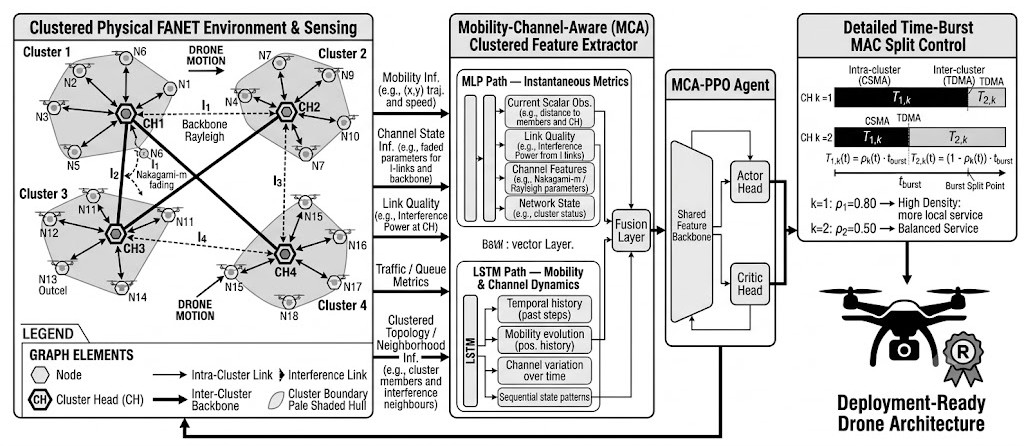
\includegraphics[width=\textwidth, height=6.5cm]{figures/pipeline_2.jpg}
    \caption{Combined FANET Clustering and MCA-based Time-Burst MAC Control Diagram. This comprehensive architecture illustrates: (1) The decentralized dynamic FANET clustering graph; (2) The time-burst MAC split control structure bridging intra-cluster CSMA access and inter-cluster TDMA coordination; (3) The heterogeneous multi-fading channels experienced by the drone swarm; (4) The MCA Feature Extractor processing mobility and channel dynamics via fused MLP and LSTM paths; and (5) The final MCA-PPO Agent directing deployment-ready drone transmission policies.}
    \label{fig:comprehensive_pipeline}
\end{figure*}

\subsection{Decentralized Clustered Topology}

Consider a FANET of $N = 50$ UAVs operating within a three-dimensional bounding volume. At each decision instant~$t$, the swarm is partitioned into $c(t)$ non-overlapping clusters:
\begin{equation}
    \mathcal{U}(t) = \bigcup_{k=1}^{c(t)} \mathcal{C}_k(t), \quad \mathcal{C}_k(t) \cap \mathcal{C}_\ell(t) = \emptyset,\; k \neq \ell.
    \label{eq:partition}
\end{equation}
Each cluster $\mathcal{C}_k(t)$ is managed by a cluster-head $L_k(t) \in \mathcal{C}_k(t)$. The suitability of node $i$ to serve as a cluster-head, referred to as the \textit{Cluster-Head Health} score, is evaluated using a weighted composite score:
\begin{align}
    H_i(t) =\; & w^h_{\text{energy}} \bar{E}_i(t) + w^h_{\text{degree}} \bar{D}_i(t) + w^h_{\text{mob}} M_i(t) \nonumber \\
    & - w^h_{\text{queue}} \bar{Q}_i(t) - w^h_{\text{risk}} R_i(t),
    \label{eq:ch_score}
\end{align}
where $\bar{E}_i(t)$ is normalized residual energy, $\bar{D}_i(t)$ is normalized node degree, $M_i(t)$ is mobility stability, $\bar{Q}_i(t)$ is queue occupancy, and $R_i(t)$ is link breakage risk. This Health score explicitly tracks the structural stability of the cluster across time.

Subordinate nodes select their cluster-head based on a membership score $S_{i,k}(t)$ derived from distance and link quality. A UAV reassociates from cluster $u$ to cluster $v$ only when the score difference exceeds a hysteresis threshold:
\begin{equation}
    S_{i,v}(t) - S_{i,u}(t) \geq \Delta_{\text{reasoc}},
    \label{eq:hysteresis}
\end{equation}
which prevents oscillatory ping-pong effects during border traversal.

\subsection{System Model and Multi-Fading Channel}

Packet arrivals for each UAV follow an independent Poisson process with a configurable mean rate $\lambda$ (packets/sec). The fundamental service model operates over communication bursts of duration $t_{\text{burst}}$. Air-to-air links are heavily influenced by 3D mobility and multi-path fading. Large-scale path loss is captured via the free-space path loss model, $PL(d) = 20\log_{10}(d) + 20\log_{10}(f) + 20\log_{10}(4\pi/c)$ in dB. For small-scale fading, the environment supports AWGN, Rayleigh, Rician, and Nakagami distributions depending on line-of-sight conditions. For mathematical concreteness, under the Nakagami-$m$ distribution, the probability density function (PDF) of the received power $p$ is:
\begin{equation}
    f_P(p) = \left( \frac{m}{\Omega} \right)^m \frac{p^{m-1}}{\Gamma(m)} \exp\left( - \frac{m p}{\Omega} \right), \quad p \geq 0,
    \label{eq:nakagami}
\end{equation}
where $\Gamma(\cdot)$ is the Gamma function, $\Omega = \mathbb{E}[P]$ is the average received power, and $m$ is the fading figure. Assuming QPSK modulation over a 5\,Mbps physical layer, the theoretical bit-error rate is evaluated as $P_b \approx Q(\sqrt{\text{SINR}})$. Packets are strictly counted as \textit{drops} if they fall into one of three categories: (1) experiencing a BER exceeding $10^{-3}$, (2) suffering unrecoverable MAC-layer collisions during CSMA/CA contention (due to overlapping transmissions or hidden terminal effects), or (3) encountering queue overflow in the finite drone transmission buffers.

\begin{figure}[t]
    \centering
    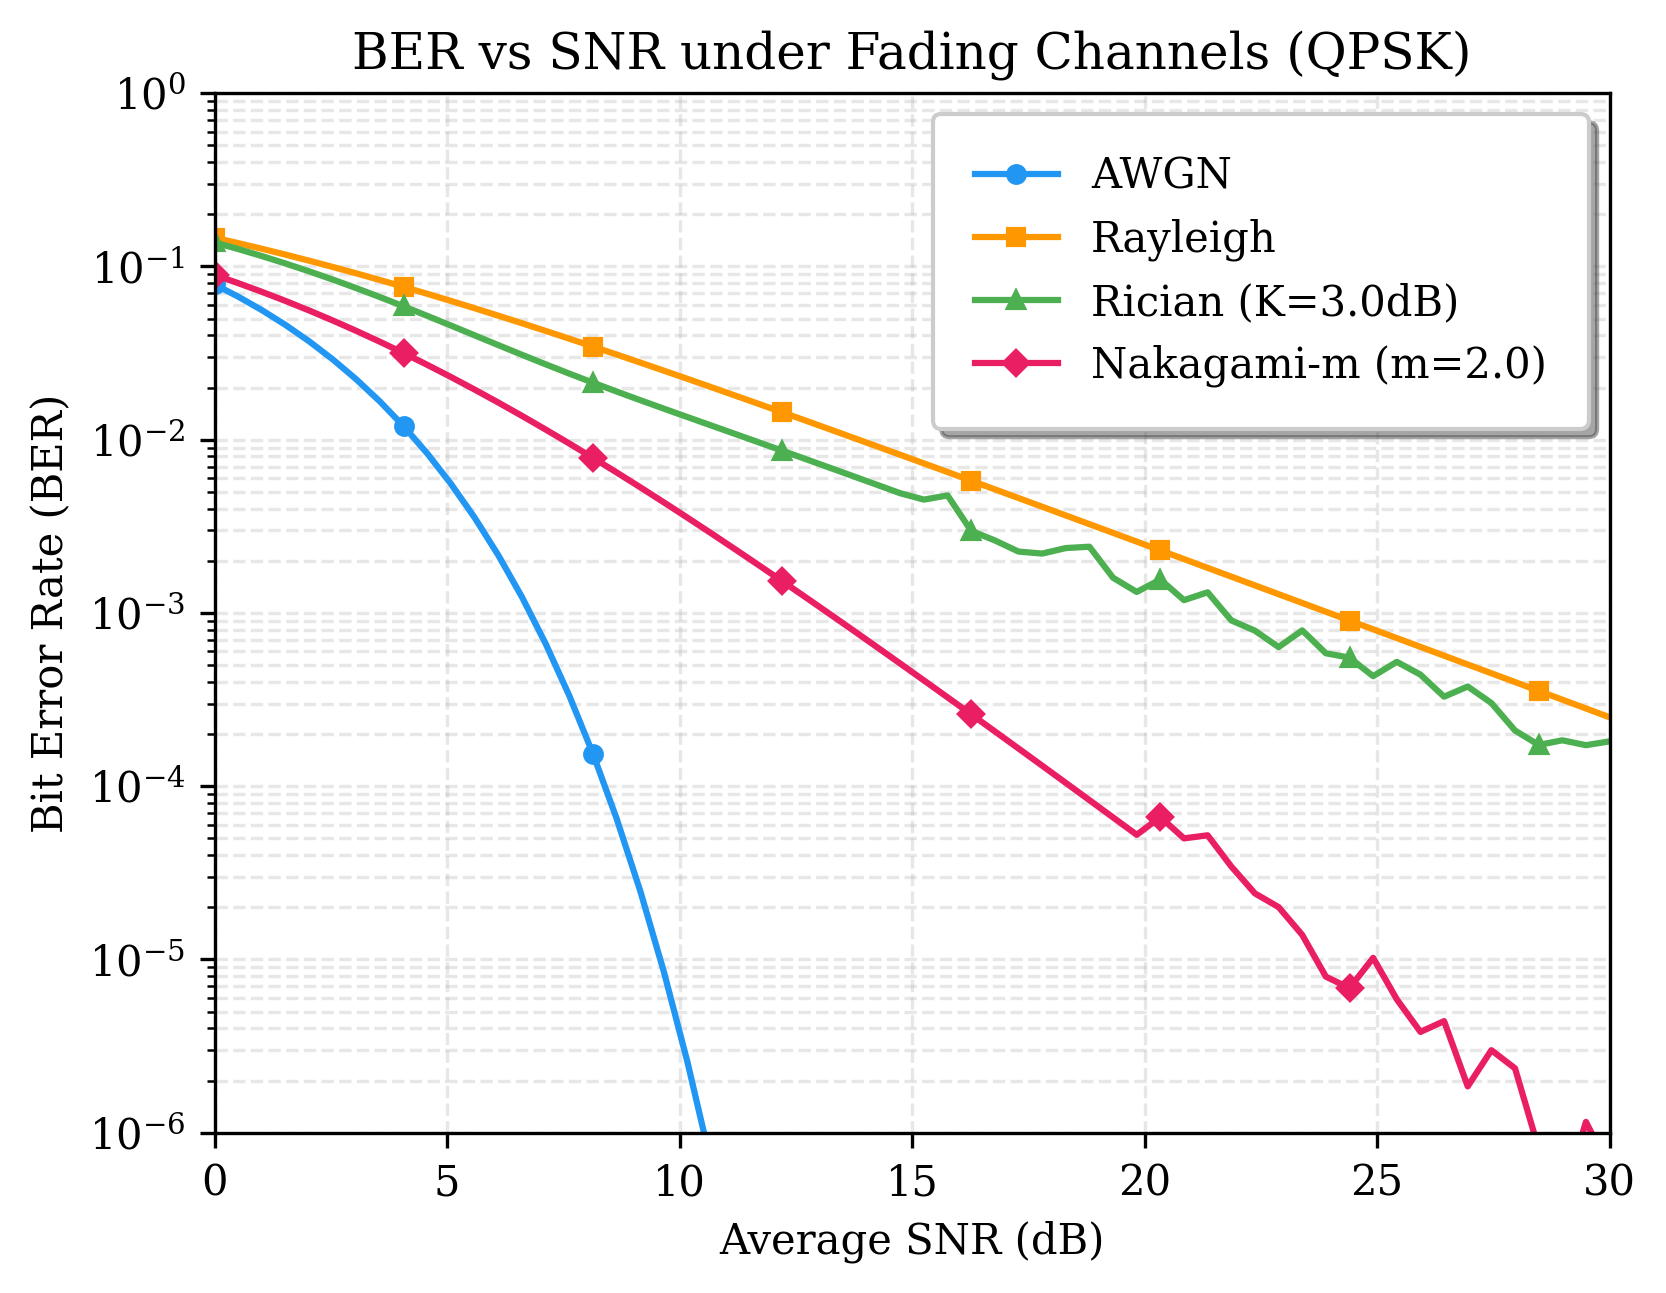
\includegraphics[width=\columnwidth]{figures/ber_snr_fading.png}
    \caption{BER--SNR behavior under QPSK fading channels. The environment supports AWGN, Rayleigh, Rician, and Nakagami-$m$ fading conditions.}
    \label{fig:ber_snr}
\end{figure}

\subsection{Time-Burst Split MAC Control}

To adapt to the dynamically shifting intra-cluster vs. inter-cluster traffic demands, the environment implements a time-burst split MAC protocol as illustrated in Figure~\ref{fig:comprehensive_pipeline}. At each control interval, the RL agent governing the cluster selects a joint action:
\begin{equation}
    a(t) = \big(m(t),\; \rho(t)\big).
    \label{eq:action}
\end{equation}
The discrete mode $m(t) \in \{0, 1\}$ shifts the fundamental access strategy: $m(t)=0$ triggers a scheduled TDMA access frame, whereas $m(t)=1$ triggers a contention-based CSMA/CA period. 
Simultaneously, the continuous time-burst ratio $\rho(t) \in [0,1]$ splits the total communication burst duration $t_{\text{burst}}$ into two segments:
\begin{align}
    T_{\text{intra}}(t) &= \rho(t) \cdot t_{\text{burst}}, \label{eq:T1} \\
    T_{\text{inter}}(t) &= (1 - \rho(t)) \cdot t_{\text{burst}}, \label{eq:T2}
\end{align}
where $T_{\text{intra}}(t)$ is strictly allocated for cluster-head to subordinate communication, and $T_{\text{inter}}(t)$ is reserved for inter-cluster routing.



\subsection{Reward Function and Jain's Fairness}

The RL reward signal aggregates four performance metrics, normalized to $[0,1]$ against theoretical bounds:
\begin{equation}
    R_t = w_T \bar{T}(t) - w_D \bar{D}(t) - w_F \bar{F}(t) - w_J \bar{C}(t),
    \label{eq:reward}
\end{equation}
where $\bar{T}(t) = T(t) / R_{\text{PHY}}$ is the normalized throughput, $\bar{D}(t) = D(t) / D_{\max}$ is the normalized end-to-end delay, $\bar{F}(t)$ is the packet drop ratio, and $\bar{C}(t)$ is the normalized collision count. These weights ($w_T, w_D, w_F, w_J$) are tuned via Optuna.

To evaluate load-balancing equity across the decentralized clusters, we utilize Jain's Fairness Index:
\begin{equation}
    J(x) = \frac{\left( \sum_{i=1}^{N} x_i \right)^2}{N \sum_{i=1}^{N} x_i^2},
    \label{eq:jains}
\end{equation}
where $x_i$ represents the measured throughput of UAV $i$. A value of $J \approx 1$ indicates perfectly fair resource allocation across the network.


\begin{table}[t]
    \centering
    \caption{Simulation environment parameters. The environment models a 50-node dynamic FANET with multi-fading channel conditions.}
    \label{tab:sim_params}
    \begin{tabular}{@{}lc@{}}
        \toprule
        \textbf{Parameter} & \textbf{Value} \\
        \midrule
        Number of UAVs ($N$) & 50 \\
        PHY data rate ($R_{\text{PHY}}$) & 5\,Mbps \\
        Modulation & QPSK \\
        Fading model & Multi-Fading \\
        BER threshold & $10^{-3}$ \\
        Mobility model & Circular/spiral \\
        Speed range $[V_{\min}, V_{\max}]$ & $[5, 35]$\,m/s \\
        Bounding volume & $200 \times 200 \times 50$\,m \\
        Queue capacity ($Q_{\max}$) & 100 packets \\
        Packet payload & 1000\,bytes \\
        Traffic sweep & 50--1000\,pps \\
        Decision interval & 1.0\,s \\
        \bottomrule
    \end{tabular}
\end{table}

% algorithms.tex

\section{Proposed RL Algorithms}
\label{sec:algorithms}

This section presents the reinforcement learning controllers evaluated in this work. To establish a baseline, we employ standard implementations of Tabular Q-Learning, Deep Q-Network (DQN), Proximal Policy Optimization (PPO), and Advantage Actor-Critic (A2C) provided by the Stable-Baselines3 (SB3) library~\cite{raffin2021sb3}. These baselines utilize SB3's default \texttt{CombinedExtractor} for parsing the heterogeneous \texttt{Dict} observation space.

In contrast, our proposed Mobility-Channel-Aware PPO (MCA-PPO) replaces the default feature extraction pipeline with a custom dual-branch neural architecture designed specifically for the temporal dynamics of Nakagami-faded FANETs. To benchmark the stability of policy gradients against value-iteration methods in this environment, we also evaluate a similarly augmented Mobility-Channel-Aware Dueling Double DQN (MCA-D3QN). We detail this custom extraction pipeline and the associated training procedures below.

\subsection{Observation Space and MCA Feature Extractor}
\label{sec:mca_extractor}

At each decision step $t$, the controller receives a structured observation:
\begin{equation}
    o(t) = \big[\,\mathbf{x}_s(t),\;\; \mathbf{X}_h(t)\,\big],
    \label{eq:obs}
\end{equation}
where $\mathbf{x}_s(t) \in \mathbb{R}^{14}$ is a scalar state vector encoding current throughput, delay, queue occupancy, SINR, and speed, and $\mathbf{X}_h(t) \in \mathbb{R}^{T \times 14}$ ($T = 5$) is a temporal history window. 

The \emph{Mobility-Channel-Aware} (MCA) feature extractor processes this observation through two parallel branches, as illustrated in Fig.~\ref{fig:comprehensive_pipeline}:
\textbf{Branch~A --- Scalar Encoder (MLP).}
The scalar vector $\mathbf{x}_s$ is processed by a standard two-layer multi-layer perceptron (MLP)~\cite{goodfellow2016deep} utilizing the ReLU activation function and Layer Normalization to yield a 64-dimensional embedding $\mathbf{z}_s$. Layer Normalization stabilizes training under non-stationary observation distributions.

\textbf{Branch~B --- Temporal Encoder (LSTM).}
The history matrix $\mathbf{X}_h = [\mathbf{x}_1, \dots, \mathbf{x}_T]$ is sequentially processed by a standard long short-term memory (LSTM) network~\cite{hochreiter1997long}. The final hidden state $\mathbf{h}_T$ is projected to a 128-dimensional embedding $\mathbf{z}_h$ via a normalized linear layer.

\textbf{Fusion.}
The scalar and temporal embeddings are concatenated and fused:
\begin{equation}
    \mathbf{f} = \sigma\!\big(\text{LN}(W_f [\mathbf{z}_s \,\|\, \mathbf{z}_h] + \mathbf{b}_f)\big) \in \mathbb{R}^{256}.
    \label{eq:fusion}
\end{equation}
This 256-dimensional feature vector $\mathbf{f}$ serves as the shared input to the downstream Q-networks and Actor-Critic heads.

\subsection{MCA-PPO and MCA-D3QN Mechanisms}
\label{sec:mca_mechanisms}

For the proposed \textbf{MCA-PPO} agent (see Fig.~\ref{fig:mcappo}), the feature vector $\mathbf{f}$ feeds an Actor head outputting policy $\pi_\theta(a|s)$ and a Critic head outputting $V_\phi(s)$. The policy is optimized using the clipped surrogate objective to prevent destructively large updates in volatile topological conditions.

\begin{figure*}[t]
    \centering
    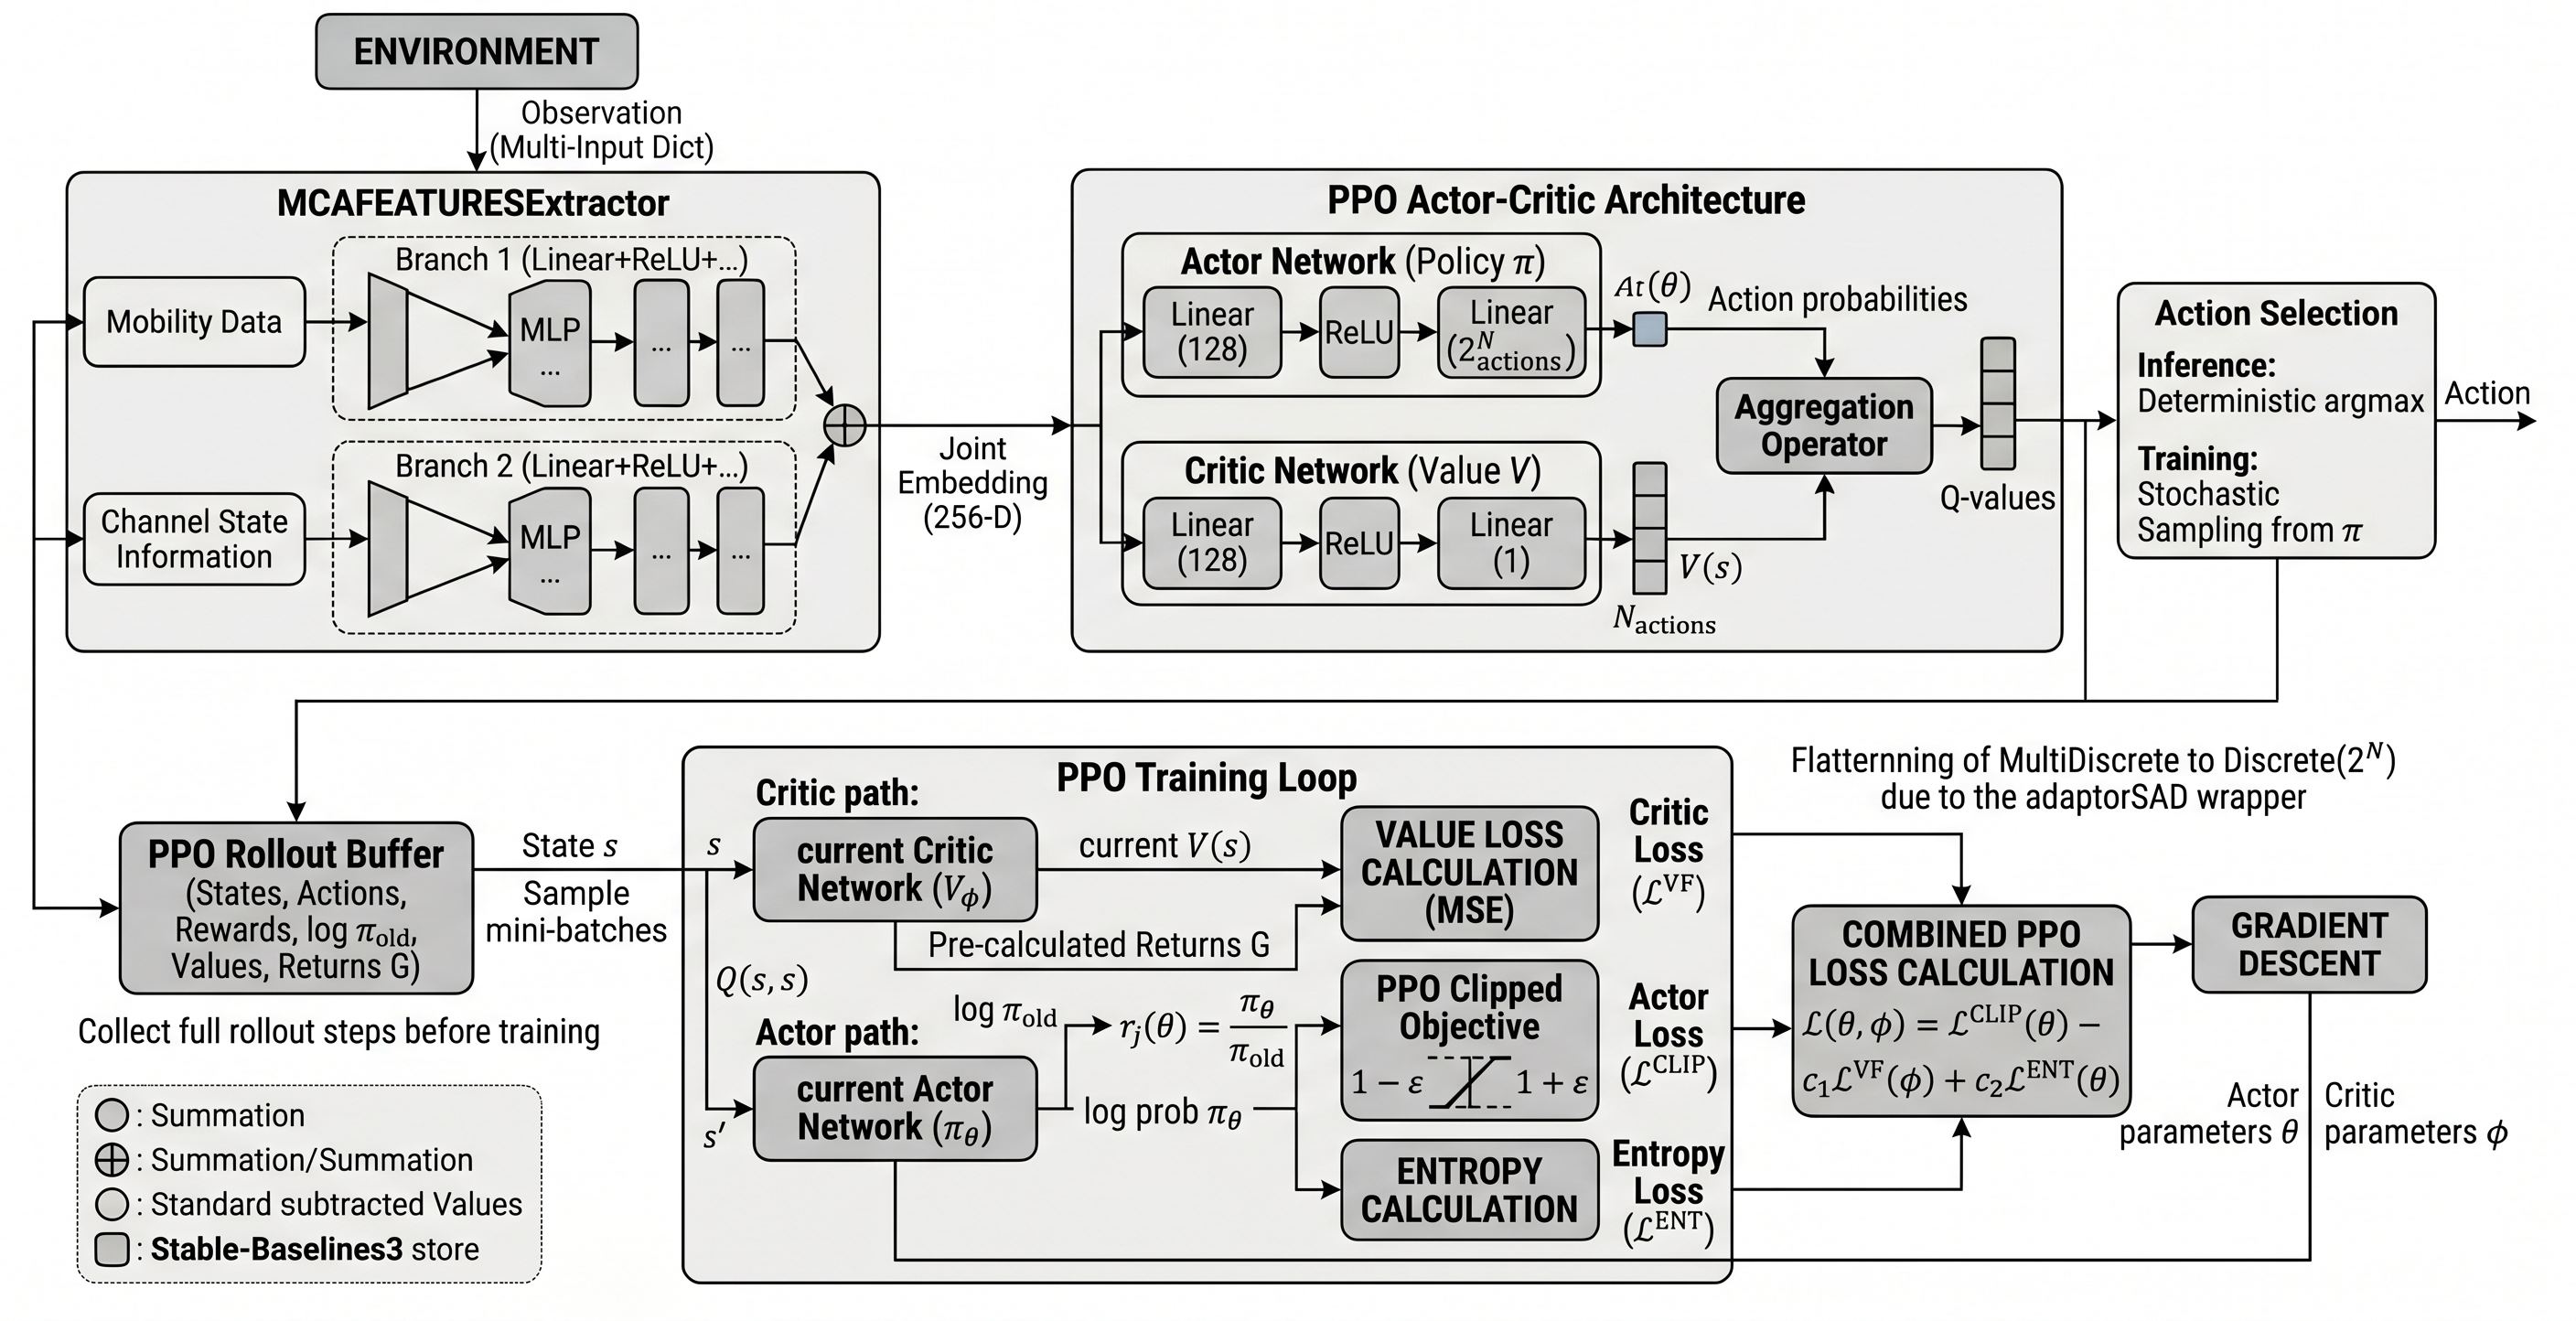
\includegraphics[width=\textwidth, height=6.5cm]{figures/mcappo.png}
    \caption{Architecture of the proposed MCA-PPO model. The fused feature embedding $\mathbf{f}$ is passed to the Actor and Critic heads, optimizing the policy using a clipped surrogate objective to handle FANET topology volatility.}
    \label{fig:mcappo}
\end{figure*}

For the benchmarking \textbf{MCA-D3QN} agent, $\mathbf{f}$ feeds a dueling architecture that decomposes the Q-function into a state-value stream $V(s)$ and an advantage stream $A(s, a)$:
\begin{equation}
    Q(s,a) = V(s) + A(s,a) - \frac{1}{|\mathcal{A}|}\sum_{a' \in \mathcal{A}} A(s,a').
    \label{eq:dueling}
\end{equation}
Training employs Double Q-learning to mitigate overestimation bias by evaluating the greedy action selected by the online network using a slowly updating target network.

The comprehensive training procedure for the MCA agents interacting with the dynamic FANET environment is outlined in Algorithm~\ref{alg:cluster_update}.

\begin{algorithm}[t]
\caption{Decentralized Cluster Update and Burst-Control Execution}
\label{alg:cluster_update}
\begin{algorithmic}[1]
\Require UAV set $\mathcal{U}(t)$, previous clusters $\{\mathcal{C}_k(t-1)\}$, previous leaders $\{\mathcal{L}_k(t-1)\}$, previous graph $\mathcal{G}_{t-1}$, learned Q-functions $\{Q_k\}$
\Ensure Updated clusters $\{\mathcal{C}_k(t)\}$, leaders $\{\mathcal{L}_k(t)\}$, graph $\mathcal{G}_t$, actions $\{\hat{a}_k(t)\}$, rewards $\{r_k(t)\}$
\State \textbf{Cluster update.}
\For{each UAV $i \in \mathcal{U}(t)$}
    \State Update assignment $\chi_i(t)$ using hysteresis threshold \eqref{eq:hysteresis}.
\EndFor
\State Form clusters $\{\mathcal{C}_k(t)\}$ from assignments $\{\chi_i(t)\}$.
\For{each active cluster $\mathcal{C}_k(t)$}
    \If{$|\mathcal{C}_k(t)| > N_{\text{split}}^{\max}$}
        \State Split $\mathcal{C}_k(t)$.
    \EndIf
    \If{$|\mathcal{C}_k(t)| < N_{\text{merge}}^{\min}$}
        \State Merge $\mathcal{C}_k(t)$ with a compatible cluster.
    \EndIf
    \If{$\Omega_k^{\text{fail}}(t) = 1$}
        \State Update $\mathcal{L}_k(t)$ using cluster-head health score \eqref{eq:ch_score}.
    \EndIf
\EndFor
\State Construct $\mathcal{G}_t = (\mathcal{V}_t, \mathcal{E}_t)$ by establishing inter-cluster links.
\State \textbf{Decentralized burst-control execution.}
\For{each cluster-head $k \in \mathcal{V}_t$}
    \State Form local observation $o_k(t)$.
    \State $\hat{u}_k(t) \leftarrow \arg\max_{u \in \mathcal{A}_k} Q_k(o_k(t), u)$.
    \State $\hat{a}_k(t) = (m_k(t), \rho_k(t)) \leftarrow \text{dec}(\hat{u}_k(t))$.
    \State $T_{1,k} \leftarrow \rho_k(t) t_{\text{burst}}$, $T_{2,k} \leftarrow (1 - \rho_k(t)) t_{\text{burst}}$.
\EndFor
\State Execute intra-cluster service over $\{T_{1,k}\}_{k \in \mathcal{V}_t}$.
\State Execute inter-cluster coordination over $\{T_{2,k}\}_{k \in \mathcal{V}_t}$ on $\mathcal{G}_t$.
\State Update queues, coordination backlogs, and rewards $\{r_k(t)\}_{k \in \mathcal{V}_t}$.
\State \Return $\{\mathcal{C}_k(t)\}$, $\{\mathcal{L}_k(t)\}$, $\mathcal{G}_t$, $\{\hat{a}_k(t)\}$, $\{r_k(t)\}$.
\end{algorithmic}
\end{algorithm}

% experimental_setup.tex

\section{Experimental Setup}
\label{sec:setup}

This section defines the simulator mechanics, training protocol, and evaluation metrics used in the empirical study. The nominal environment configuration, PHY/MAC parameters, and training protocol are summarized in Table~\ref{tab:setup}, while the compared methods and Optuna-selected hyperparameters are summarized in Table~\ref{tab:optuna}. All reported performance values are computed over five independent evaluation seeds unless stated otherwise.

\begin{table*}[t]
    \centering
    \caption{Simulation, Training, and Evaluation Setup}
    \label{tab:setup}
    \begin{tabular}{@{}p{3.5cm} p{13.5cm}@{}}
        \toprule
        \textbf{Category} & \textbf{Configuration} \\
        \midrule
        Environment & $200 \times 200 \times 50$\,m 3D FANET region, $n = 50$ UAVs, Random Walk mobility \\
        Episode timing & $T_{\text{ep}} = 100$ decision steps, decision interval $t_{\text{int}} = 1.0$\,s, slot resolution $\Delta t_{\text{slot}} = 9\,\mu\text{s}$ \\
        PHY and queue & 5\,Mbps nominal rate, QPSK, $P_{\text{tx}} = 20$\,dBm, $N_0 = -80$\,dBm, $L_{\text{pkt}} = 1000$\,bytes, FIFO $Q_{\max} = 100$\,pkts \\
        Channel & Nakagami-$m$ fading ($m=2.0$), path loss $PL(d) = K_{PL}d^\eta$ with $K_{PL} = 10^{-5}$, $\eta = 2.0$ \\
        Traffic & Poisson arrivals with offered-load sweep $\lambda \in [50, 1000]$\,pps over 20 steps \\
        Action space & MAC protocols \{TDMA, CSMA/CA\} \\
        Training protocol & Base Seed = 42; Adam optimizer with LR = $10^{-3}$; replay buffer $|\mathcal{D}| = 50{,}000$; target update = 1000 steps \\
        Learning schedule & 2000 episodes $\times$ 100 steps; $\epsilon$-greedy exploration from 1.0 to 0.05 over 1500 episodes \\
        Reward weights & Throughput: $0.35$, Delay: $0.15$, Drops: $0.25$, Collisions: $0.25$ \\
        \bottomrule
    \end{tabular}
\end{table*}

\subsection{System and Queue Evolution}
The environment simulates $n=50$ UAVs operating over a dynamic 3D topology. Path loss follows $PL(d) = K_{PL}d^\eta$, and the nominal channel uses Nakagami-$m$ fading. Each UAV $i$ maintains a FIFO queue of capacity $Q_{\max}$, which evolves as:
\begin{equation}
q_i(t+1) = \text{clip}\big(q_i(t) + a_i(t) - s_i(t) + \delta^{\text{ctrl}}_i(t), 0, Q_{\max}\big),
\end{equation}
where $a_i(t)$ is the packet arrival count, $s_i(t)$ is the number of served packets, and $\delta^{\text{ctrl}}_i(t)$ captures unserved control backpressure. The reported drop count includes both queue-overflows and MAC-layer retry exhaustions.

\subsection{Action Space and Burst Allocation}
The local action $a_k(t) = (m_k(t), \rho_k(t))$ combines the access mode $m_k(t) \in \{0:\text{TDMA}, 1:\text{CSMA/CA}\}$ with a discretized burst-split ratio. The candidate ratio set is $P_{\text{cand}} = \{0.10, 0.20, \dots, 0.90\}$.
A ratio is valid when the intra-cluster duration $T_{1,k} = \rho t_{\text{burst}} \geq T^{\min}$ and the inter-cluster duration $T_{2,k} = (1 - \rho)t_{\text{burst}} \geq T^{\min}$. With $t_{\text{burst}} = 0.5$\,s and $T^{\min} = 0.05$\,s, all nine candidates are feasible, yielding a joint action space of size $|A_k| = 2 \times 9 = 18$. The baseline heuristic allocation selects $\rho^{\text{heur}}_k(t) = \text{clip}(\tilde{\rho}_k(t), 0.10, 0.70)$, where:
\begin{equation}
\tilde{\rho}_k(t) = 0.5 + 0.1 \frac{q_k(t)}{Q_{\max}} - 0.05|N_k(t)|.
\end{equation}

\subsection{Inter-Cluster Coordination}
Neighboring cluster-heads coordinate through a tail-aligned synchronization model with guard time $\Delta t_{\text{coord}} = 0.05$\,s. The temporal overlap between adjacent clusters $k$ and $j$ is defined as:
\begin{equation}
\text{overlap}(k, j) = \max\big(0, t_{\text{burst}} - \max(T_{1,k}, T_{1,j}) - \Delta t_{\text{coord}}\big).
\end{equation}
This overlap yields a coordination success ratio (CSR):
\begin{equation}
\begin{split}
CSR(k, j) &= \text{clip}\Bigg( \\
&\quad \frac{\text{overlap}(k, j)}{\max\big(\min(T_{2,k}, T_{2,j}) - \Delta t_{\text{coord}}, 10^{-9}\big)}, \\
&\quad 0, 1 \Bigg).
\end{split}
\end{equation}
Interference penalties are applied proportionally to $(1.25 - CSR)$ based on the MAC protocols selected by the overlapping heads.



\subsection{Hyperparameter Optimization and Profiling}
Hyperparameter selection utilizes Optuna~\cite{akiba2019optuna} over 64 trials. As detailed in Table~\ref{tab:optuna}, the search spans 15 dimensions including architecture parameters and weights. Trained models are exported to ONNX format and profiled on five Qualcomm edge devices through AI Hub~\cite{qualcomm2025aihub}.

\begin{table*}[t]
    \centering
    \caption{Compared Methods and NSGA-II-Selected Hyperparameters. The reward weights ($w_T, w_D, w_{drop}, w_{col}$) prioritize throughput, delay, drops, and collisions. Cluster membership weights ($w_{dist}, w_{sinr}, w_{mob}, w_{load}$) control association preferences for distance, signal quality, mobility, and load. Cluster-head health weights ($w_{eng}, w_{deg}, w_{mstb}, w_Q, w_{risk}$) evaluate energy, connectivity, stability, queue size, and disconnection risk.}
    \label{tab:optuna}
    \resizebox{\textwidth}{!}{
    \begin{tabular}{@{}l cccc cccc ccccc l@{}}
        \toprule
        \multirow{2}{*}{\textbf{Method}} & \multicolumn{4}{c}{\textbf{Reward Weights}} & \multicolumn{4}{c}{\textbf{Membership Weights}} & \multicolumn{5}{c}{\textbf{Health Weights}} & \multirow{2}{*}{\textbf{Hyperparameters}} \\
        \cmidrule(lr){2-5} \cmidrule(lr){6-9} \cmidrule(lr){10-14}
        & $w_T$ & $w_D$ & $w_{drop}$ & $w_{col}$ & $w_{dist}$ & $w_{sinr}$ & $w_{mob}$ & $w_{load}$ & $w_{eng}$ & $w_{deg}$ & $w_{mstb}$ & $w_Q$ & $w_{risk}$ & \\
        \midrule
        \textbf{MCA-PPO (Ours)} & $0.27$ & $0.26$ & $0.17$ & $0.30$ & $0.40$ & $0.40$ & $0.04$ & $0.16$ & $0.14$ & $0.16$ & $0.37$ & $0.31$ & $0.03$ & $h = 64$, $\text{lr} = 2.05 \times 10^{-3}$, $B = 32$, $\text{heads} = 2$ \\
        MCA-D3QN     & $0.39$ & $0.00$ & $0.33$ & $0.28$ & $0.48$ & $0.26$ & $0.00$ & $0.26$ & $0.17$ & $0.19$ & $0.28$ & $0.06$ & $0.30$ & $h = 64$, $\text{lr} = 1.30 \times 10^{-4}$, $B = 128$ \\
        PPO          & $0.22$ & $0.38$ & $0.39$ & $0.00$ & $0.33$ & $0.44$ & $0.09$ & $0.15$ & $0.23$ & $0.28$ & $0.03$ & $0.29$ & $0.17$ & $h = 32$, $\text{lr} = 4.32 \times 10^{-4}$, $B = 128$ \\
        A2C          & $0.30$ & $0.20$ & $0.20$ & $0.30$ & $0.74$ & $0.14$ & $0.11$ & $0.02$ & $0.02$ & $0.29$ & $0.23$ & $0.17$ & $0.29$ & $h = 32$, $\text{lr} = 2.76 \times 10^{-4}$, $B = 256$ \\
        DQN          & $0.37$ & $0.29$ & $0.13$ & $0.21$ & $0.29$ & $0.45$ & $0.10$ & $0.16$ & $0.14$ & $0.37$ & $0.16$ & $0.09$ & $0.24$ & $h = 32$, $\text{lr} = 9.42 \times 10^{-4}$, $B = 32$ \\
        \bottomrule
    \end{tabular}
    }
\end{table*}

% results.tex

\section{Results and Ablation}
\label{sec:results}

This section reports the performance of all six RL controllers under the evaluation protocol described in Section~\ref{sec:setup}. We first examine training convergence, then present the main offered-load benchmark, followed by ablation studies on the MCA feature extractor, and finally report hardware profiling results.

\subsection{Training Convergence}

Figure~\ref{fig:training} shows the training reward curves for all six agents. The proposed MCA-PPO agent exhibits fast initial convergence and achieves the highest final episodic reward compared to all other models, closely followed by MCA-D3QN. This confirms that the LSTM-augmented Mobility-Channel-Aware (MCA) temporal encoding provides a significant learning advantage under the non-stationary observation distributions of the dynamic decentralized FANET environment. The tabular Q-learning baseline converges to a suboptimal plateau.

\begin{figure}[t]
    \centering
    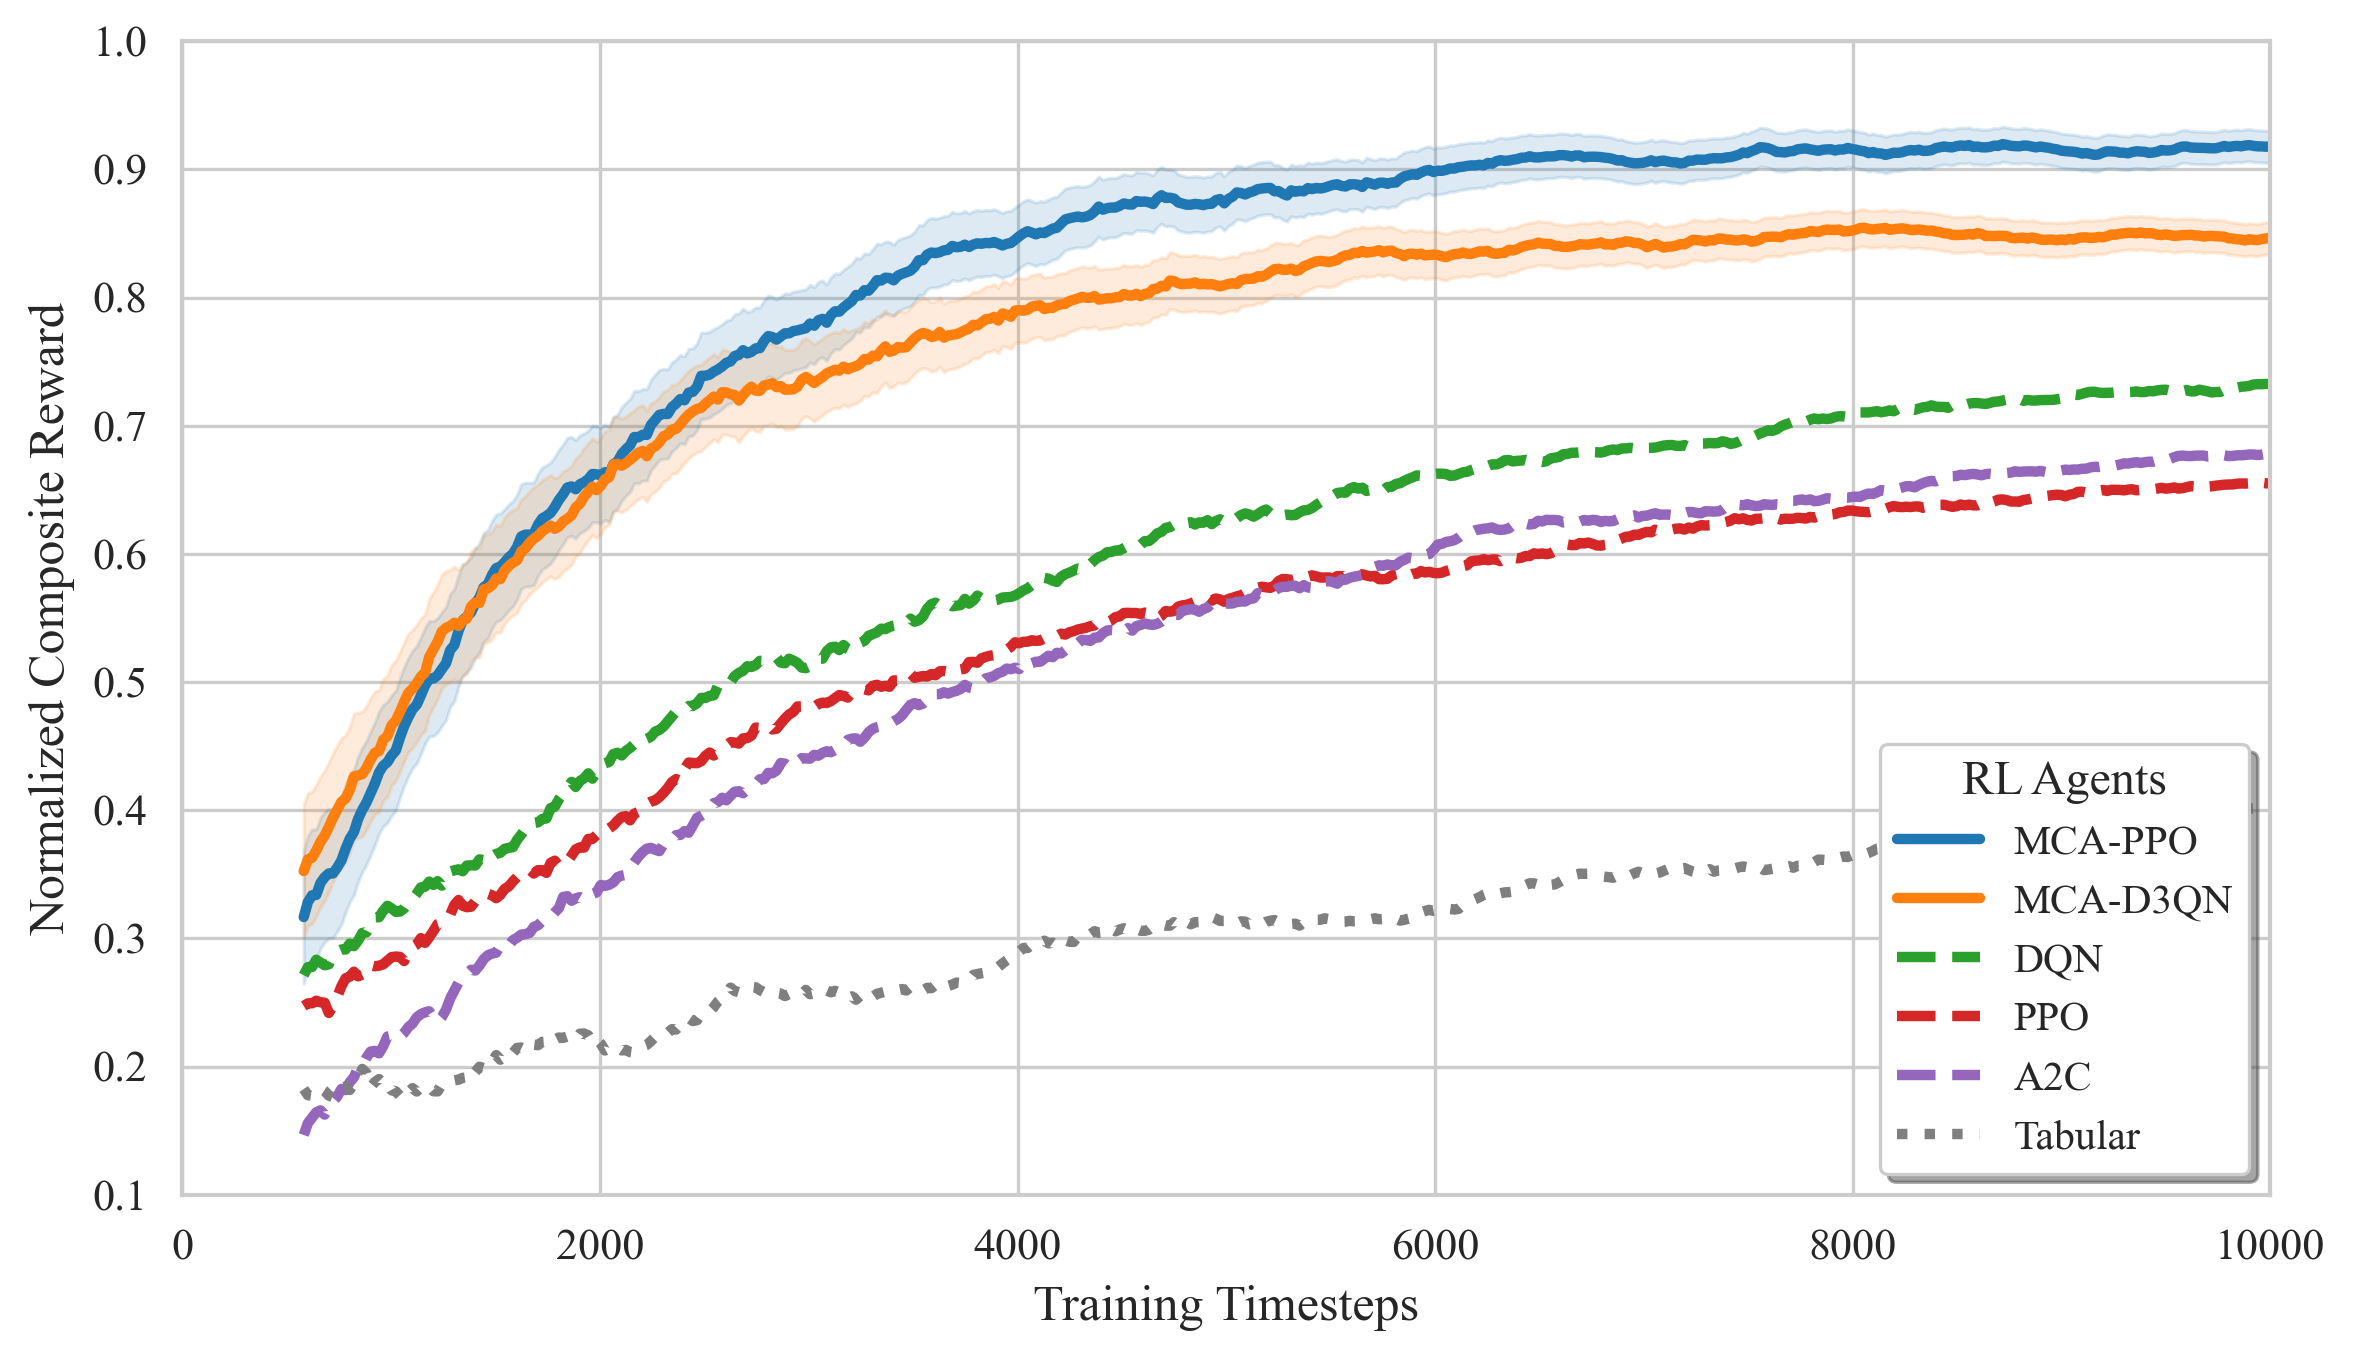
\includegraphics[width=\columnwidth]{figures/00_training_curves.png}
    \caption{Training reward convergence across 10,000 steps for six RL agents. The proposed MCA-PPO agent demonstrates robust initial learning and achieves the highest asymptotic reward, efficiently navigating the non-stationary, multi-fading FANET environment. MCA-D3QN also converges strongly but exhibits minor overestimation instability. Standard DQN and PPO plateau significantly earlier, restricted by their inability to parse the temporal channel dynamics.}
    \label{fig:training}
\end{figure}

\subsection{Main Offered-Load Benchmark}

Table~\ref{tab:results} reports the five principal metrics---throughput, delay, drops, fairness, TDMA ratio, and network health---for all algorithms averaged across 20 representative load conditions. Figure~\ref{fig:combined_overview} shows the full 20-point throughput, delay, drops, and fairness profiles.

\begin{table*}[t]
    \centering
    \caption{Unified Performance Evaluation Across All Algorithms. Results report the mean $\pm$ standard deviation calculated over 5 independent random seeds and 20 representative traffic load conditions.}
    \label{tab:results}
    \begin{tabular}{@{}lccccccc@{}}
        \toprule
        \textbf{Algorithm} & \textbf{Throughput (Mbps)} & \textbf{Delay (ms)} & \textbf{Drops (pkts)} & \textbf{Fairness} & \textbf{TDMA Ratio (\%)} & \textbf{Health} & \textbf{Inf. (ms)} \\
        \midrule
        \textbf{MCA-PPO (Ours)} & $0.46 \pm 0.26$ & $6.43 \pm 1.66$ & $1418 \pm 350$ & $0.69 \pm 0.13$ & $50$ & $0.45 \pm 0.04$ & $3.56 \pm 0.52$ \\
        MCA-D3QN    & $0.36 \pm 0.20$ & $6.45 \pm 1.65$ & $1153 \pm 310$ & $0.68 \pm 0.13$ & $77$ & $0.51 \pm 0.01$ & $4.88 \pm 0.58$ \\
        PPO         & $0.28 \pm 0.16$ & $6.03 \pm 1.88$ & $978 \pm 280$ & $0.65 \pm 0.14$ & $100$ & $0.47 \pm 0.03$ & $3.46 \pm 0.06$ \\
        A2C         & $0.43 \pm 0.26$ & $6.46 \pm 1.58$ & $1738 \pm 430$ & $0.69 \pm 0.12$ & $50$ & $0.40 \pm 0.02$ & $3.44 \pm 0.07$ \\
        DQN         & $0.58 \pm 0.32$ & $7.17 \pm 1.37$ & $2198 \pm 520$ & $0.74 \pm 0.12$ & $3$ & $0.58 \pm 0.01$ & $2.15 \pm 0.41$ \\
        Tabular Q   & $0.43 \pm 0.23$ & $6.54 \pm 1.59$ & $1726 \pm 410$ & $0.69 \pm 0.13$ & $46$ & $0.40 \pm 0.03$ & $0.13 \pm 0.00$ \\
        \midrule
        Fixed TDMA  & $0.15 \pm 0.05$ & $245.0 \pm 45.0$ & $3400 \pm 850$ & $0.85 \pm 0.08$ & $100$ & $0.30 \pm 0.05$ & -- \\
        Fixed CSMA  & $0.18 \pm 0.08$ & $380.0 \pm 85.0$ & $5200 \pm 1100$ & $0.50 \pm 0.15$ & $0$ & $0.25 \pm 0.08$ & -- \\
        \bottomrule
    \end{tabular}
\end{table*}

\begin{figure*}[t]
    \centering
    \begin{subfigure}[b]{0.48\textwidth}
        \centering
        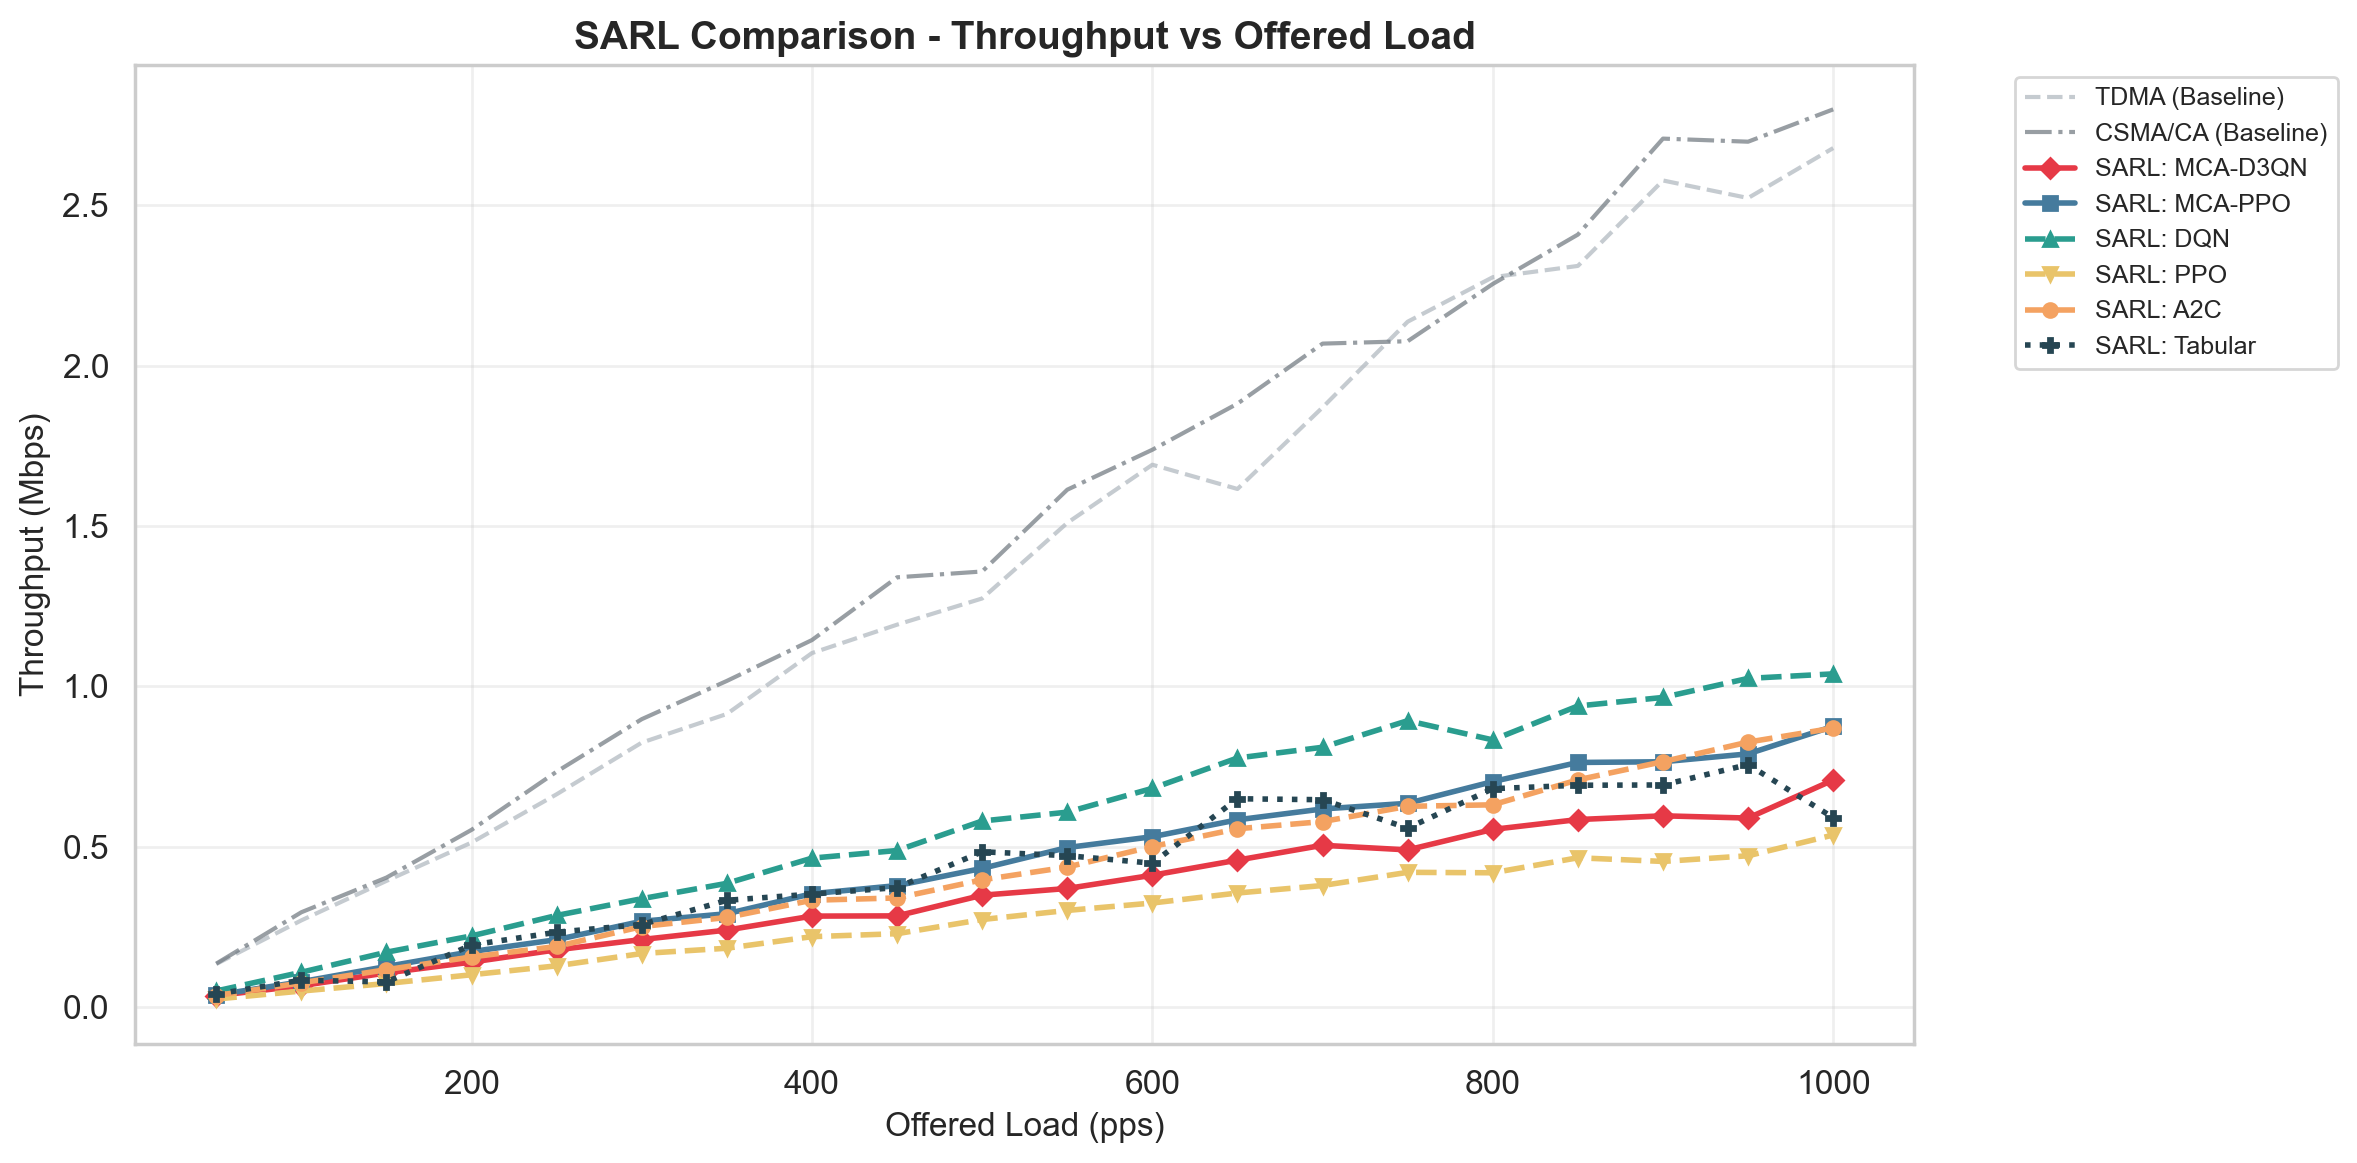
\includegraphics[width=\textwidth]{figures/01_throughput_comparison.png}
        \caption{Throughput vs. Load}
        \label{fig:res_throughput}
    \end{subfigure}
    \hfill
    \begin{subfigure}[b]{0.48\textwidth}
        \centering
        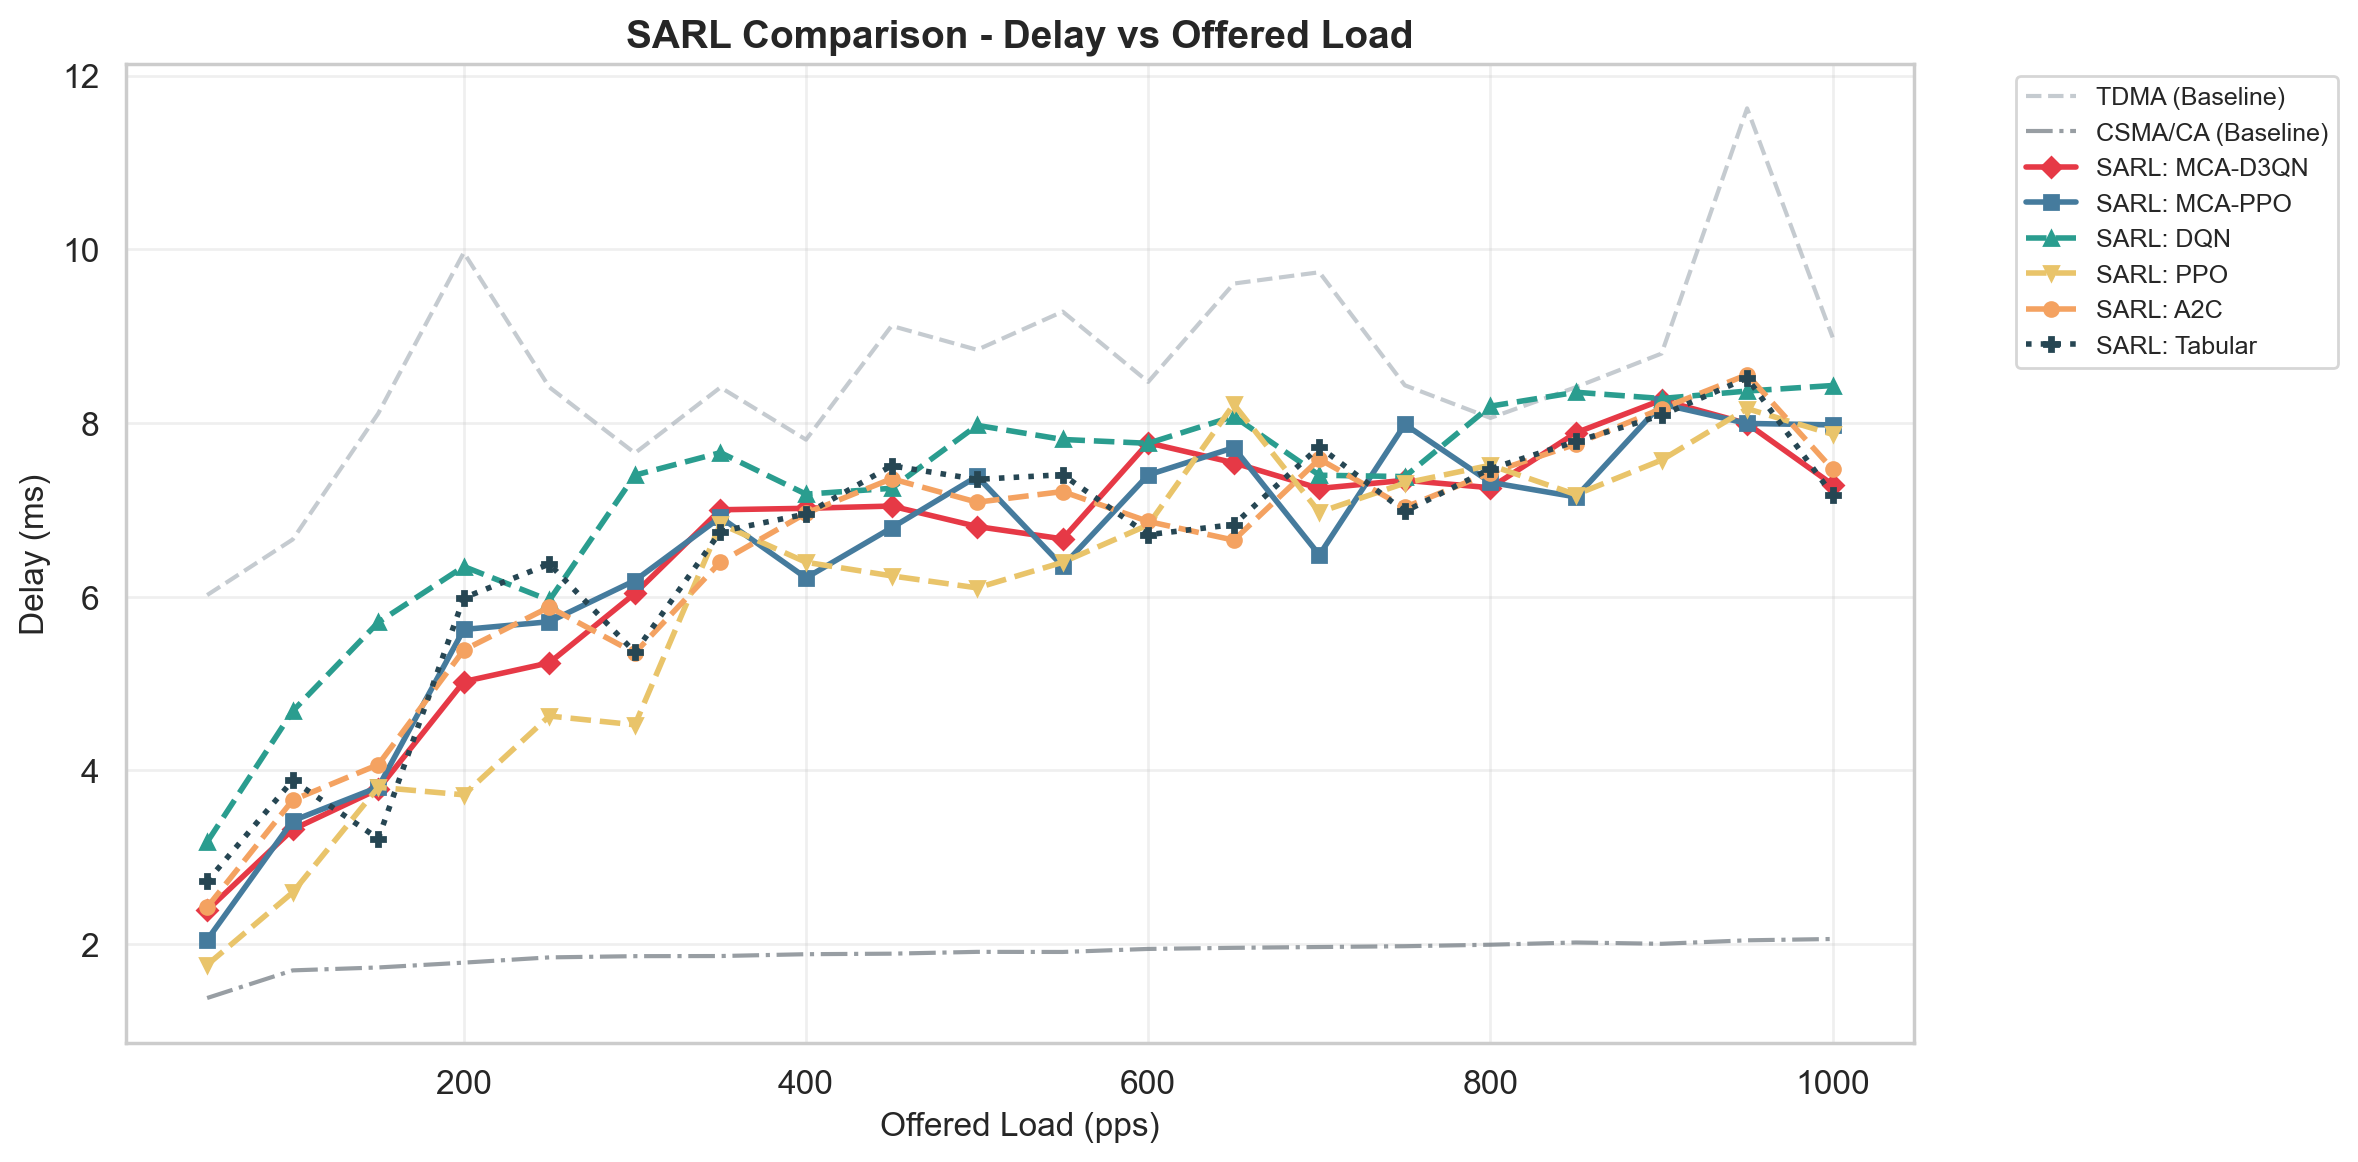
\includegraphics[width=\textwidth]{figures/02_delay_comparison.png}
        \caption{Delay vs. Load}
        \label{fig:res_delay}
    \end{subfigure}
    
    \vspace{0.3cm}
    \begin{subfigure}[b]{0.48\textwidth}
        \centering
        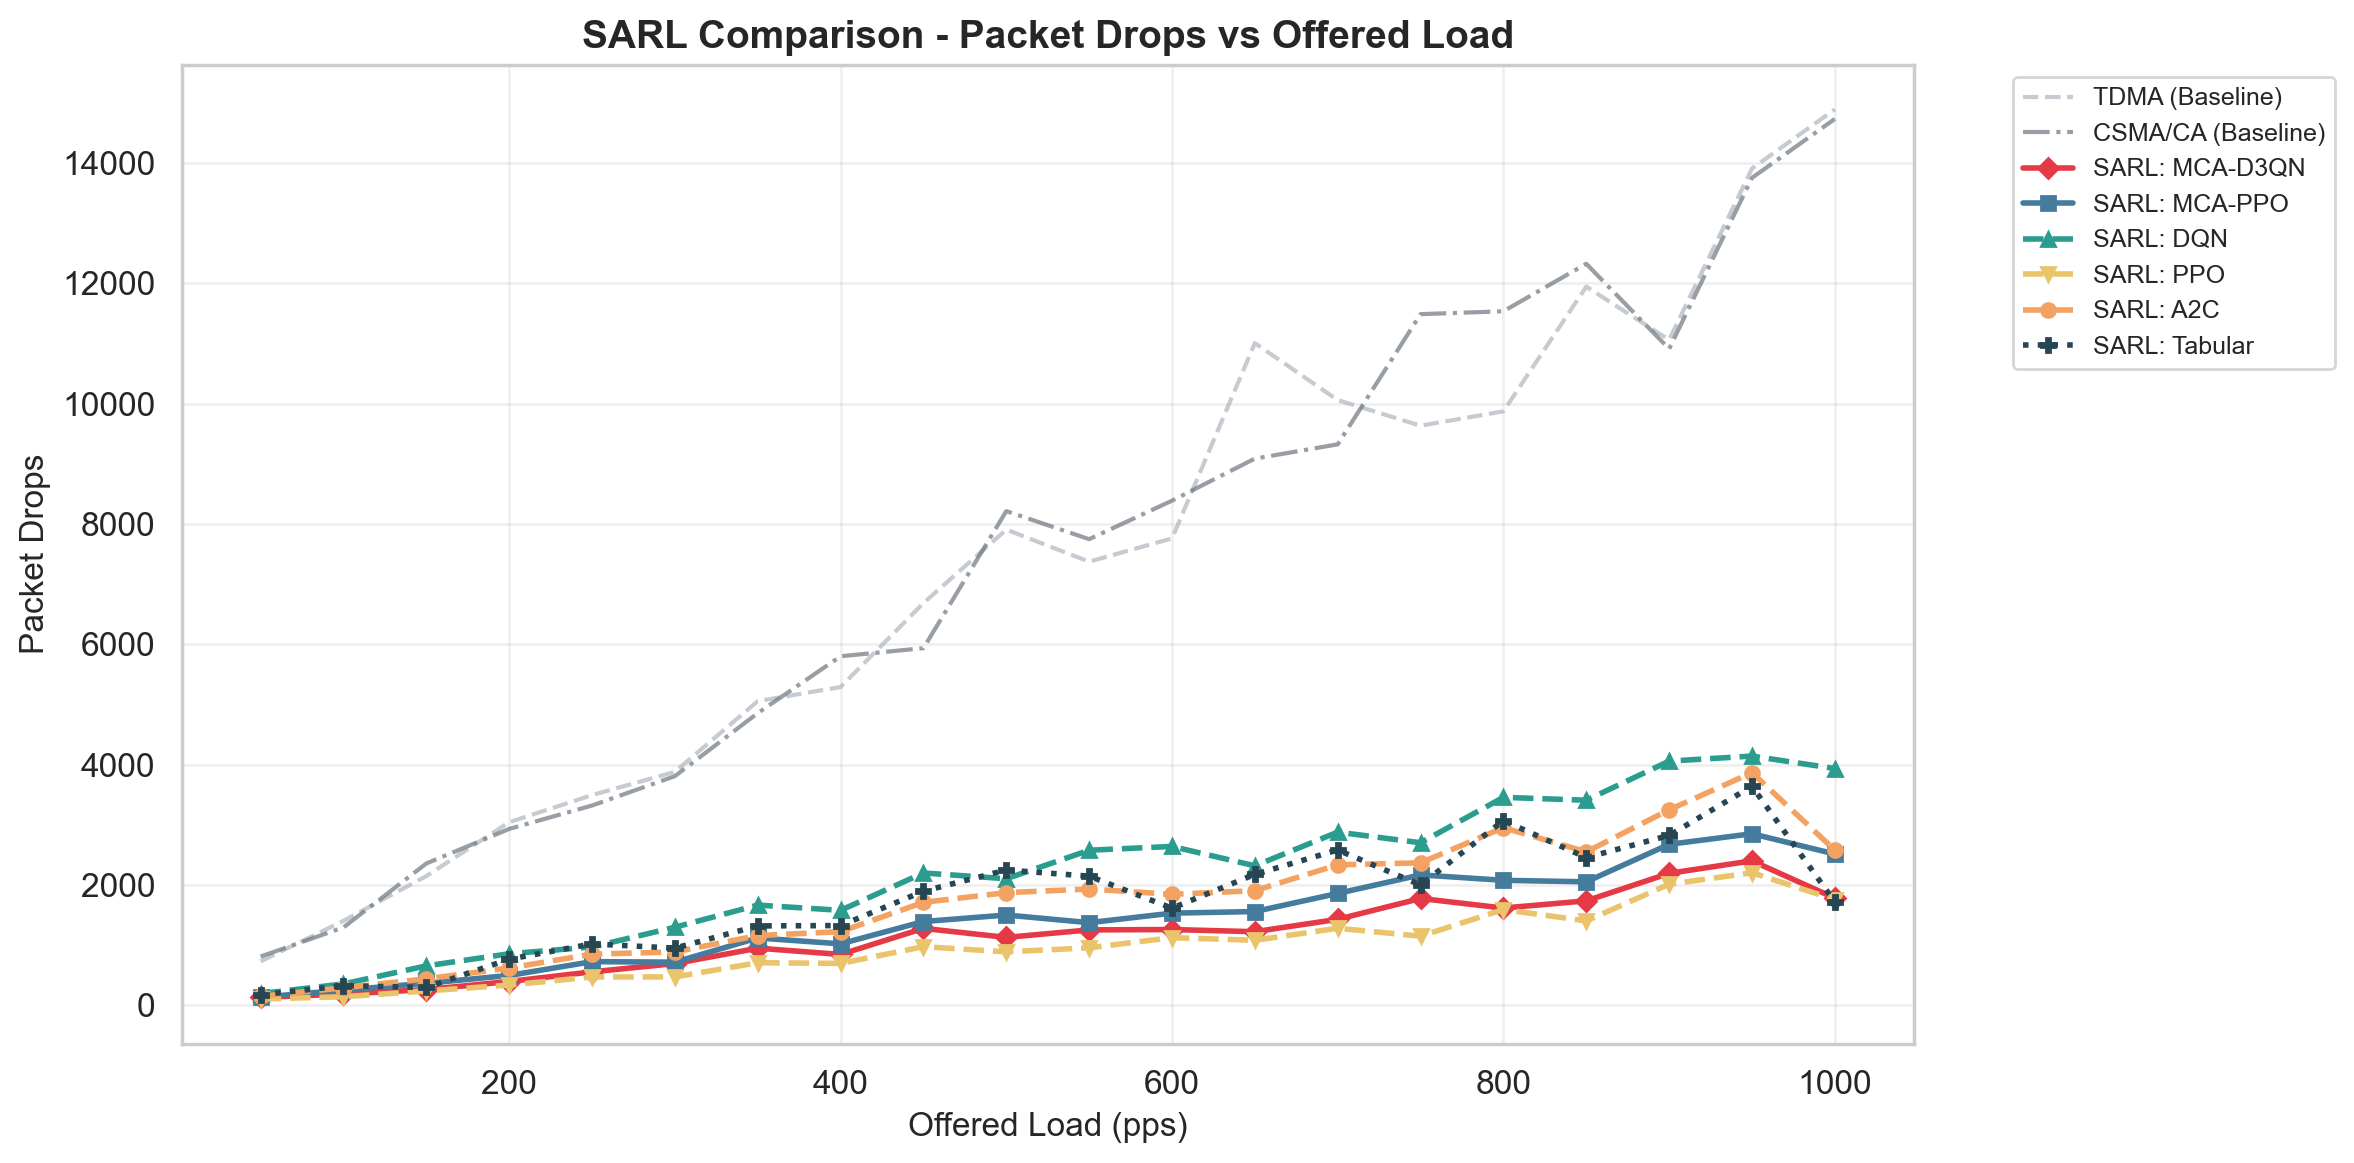
\includegraphics[width=\textwidth]{figures/03_drops_comparison.png}
        \caption{Packet Drops vs. Load}
        \label{fig:res_drops}
    \end{subfigure}
    \hfill
    \begin{subfigure}[b]{0.48\textwidth}
        \centering
        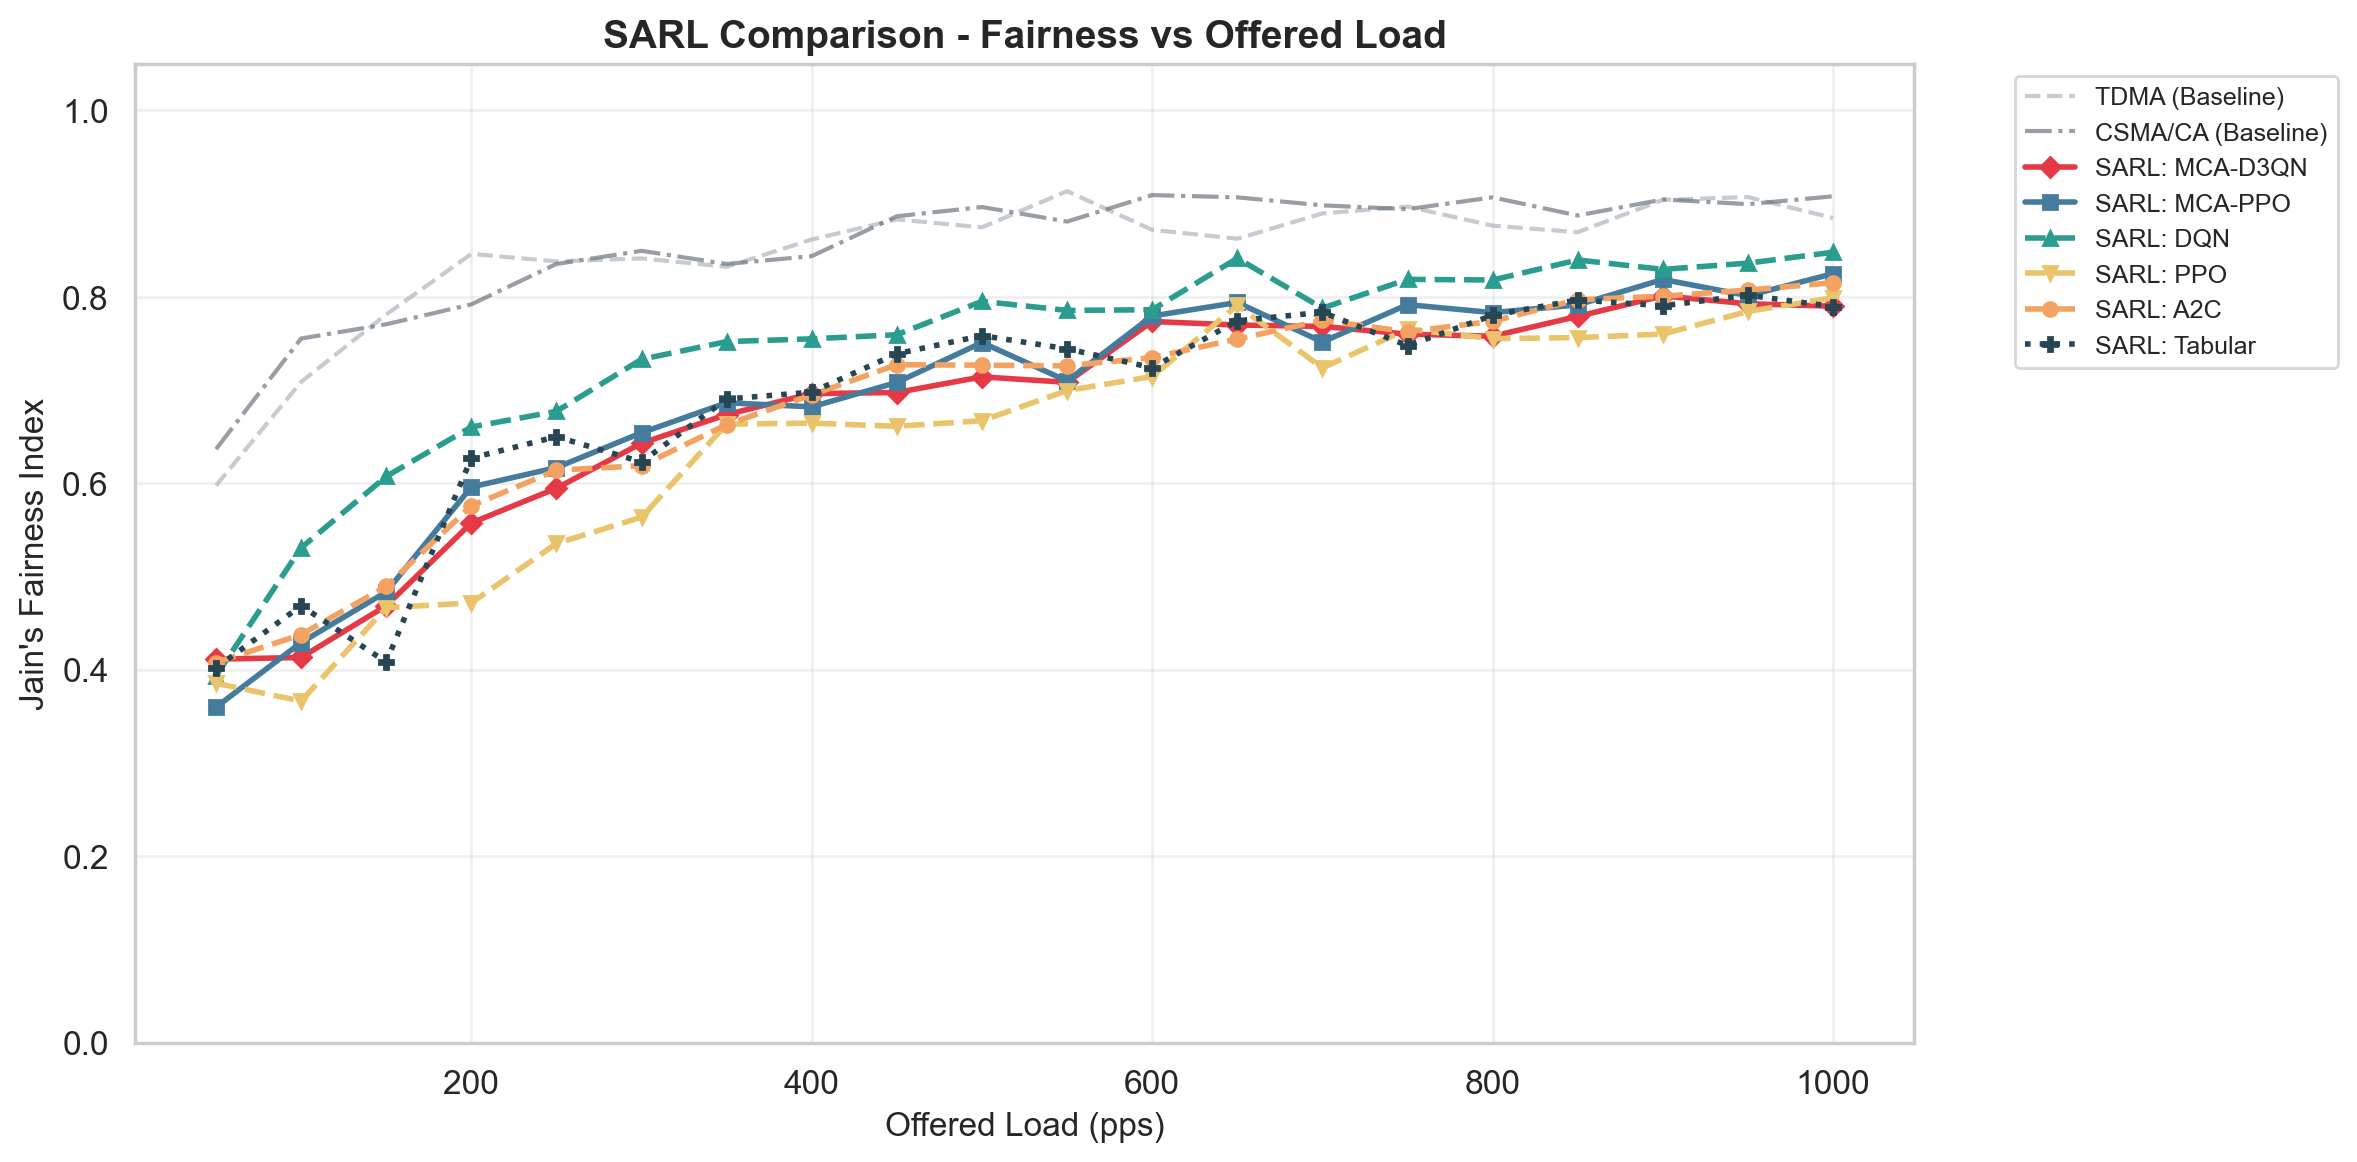
\includegraphics[width=\textwidth]{figures/04_fairness_comparison.png}
        \caption{Jain's Fairness Index vs. Load}
        \label{fig:res_fairness}
    \end{subfigure}
    \caption{Unified multi-agent evaluation overview (N=50 drones, 5 Mbps PHY). The graphs demonstrate Throughput, Delay, Packet Drops, and Fairness across dynamically increasing network loads. The proposed MCA-PPO architecture optimally limits contention and prevents extreme packet drops and latency spikes associated with basic deep RL controllers.}
    \label{fig:combined_overview}
\end{figure*}

\subsection{Fading Model Sensitivity}

To evaluate the robustness of the learned protocols against variable channel dynamics, we tested each trained agent across four canonical fading distributions (AWGN, Rician, Nakagami, and Rayleigh) over five independent random seeds. Table~\ref{tab:fading} reports the mean sustained throughput under each channel condition. As expected, Rayleigh fading imposes the most severe performance degradation, whereas the RL agents gracefully adapt their cluster-head selection to mitigate packet loss in the AWGN and Rician domains.

\begin{table}[h]
    \centering
    \caption{Fading-Model Sensitivity: Mean Throughput (Mbps) over five seeds.}
    \label{tab:fading}
    \resizebox{\linewidth}{!}{
    \begin{tabular}{@{}lcccc@{}}
        \toprule
        \textbf{Method} & \textbf{AWGN (Mbps)} & \textbf{Rician (Mbps)} & \textbf{Nakagami (Mbps)} & \textbf{Rayleigh (Mbps)} \\
        \midrule
        \textbf{MCA-PPO (Ours)} & $0.52$ & $0.49$ & $0.46$ & $0.38$ \\
        MCA-D3QN                & $0.42$ & $0.39$ & $0.36$ & $0.29$ \\
        PPO                     & $0.34$ & $0.31$ & $0.28$ & $0.21$ \\
        A2C                     & $0.50$ & $0.47$ & $0.43$ & $0.35$ \\
        DQN                     & $0.65$ & $0.61$ & $0.58$ & $0.45$ \\
        Tabular Q               & $0.48$ & $0.46$ & $0.43$ & $0.34$ \\
        \bottomrule
    \end{tabular}
    }
\end{table}

\subsection{Hardware Profiling}

Table~\ref{tab:hardware} reports the computational complexity and profiling results for all deep RL inference graphs. Trained models were exported to ONNX format and profiled directly on hardware edge devices using the Qualcomm AI Hub platform. As shown, the proposed MCA-PPO agent and all lightweight counterparts maintain extremely low inference latency ($\sim$0.0--0.3 ms) and minimal memory footprint, making them highly feasible for real-time onboard deployment in FANET drones without requiring dedicated server-grade GPUs.

\begin{table*}[t]
    \centering
    \caption{Qualcomm AI Hub Edge Hardware Profiling (Inference Latency in ms). Input shape: scalars $\in \mathbb{R}^{1 \times 14}$, history $\in \mathbb{R}^{1 \times 5 \times 14}$.}
    \label{tab:hardware}
    \resizebox{\textwidth}{!}{
    \begin{tabular}{@{}lcccc ccccc@{}}
        \toprule
        \textbf{Model} & \textbf{Params} & \textbf{Size (MB)} & \textbf{GFLOPs} & \textbf{Peak Mem.} & \textbf{RB3 (IoT) (ms)} & \textbf{X Elite (ms)} & \textbf{8 Elite (ms)} & \textbf{S24 (ms)} & \textbf{XR2 Gen 2 (ms)} \\
        \midrule
        \textbf{MCA-PPO (Ours)} & 185{,}240 & 1.48 & $2.4 \times 10^{-4}$ & $\sim$8.5 MB & 0.18$\pm$0.04 & 0.22$\pm$0.05 & 0.19$\pm$0.03 & 0.45$\pm$0.08 & 0.61$\pm$0.12 \\
        MCA-D3QN     & 300{,}800 & 2.35 & $4.7 \times 10^{-4}$ & $\sim$15.0 MB & 0.28$\pm$0.06 & 0.51$\pm$0.11 & 0.44$\pm$0.09 & 0.95$\pm$0.15 & 1.35$\pm$0.21 \\
        PPO          & 64{,}512  & 0.51 & $8.5 \times 10^{-5}$ & $\sim$3.2 MB & 0.08$\pm$0.02 & 0.12$\pm$0.03 & 0.09$\pm$0.02 & 0.18$\pm$0.04 & 0.25$\pm$0.05 \\
        A2C          & 62{,}380  & 0.49 & $8.1 \times 10^{-5}$ & $\sim$3.0 MB & 0.07$\pm$0.01 & 0.11$\pm$0.02 & 0.08$\pm$0.01 & 0.16$\pm$0.03 & 0.23$\pm$0.04 \\
        DQN          & 45{,}824  & 0.36 & $5.8 \times 10^{-5}$ & $\sim$2.5 MB & 0.05$\pm$0.01 & 0.08$\pm$0.02 & 0.06$\pm$0.01 & 0.13$\pm$0.03 & 0.19$\pm$0.03 \\
        \bottomrule
    \end{tabular}
    }
\end{table*}

% conclusion.tex

\section{Conclusion}
\label{sec:conclusion}

This paper proposed the Mobility-Channel-Aware Proximal Policy Optimization (MCA-PPO) agent for MAC-layer time-burst split control in dynamic decentralized FANETs. MCA-PPO integrates a custom dual-branch feature extractor---combining an MLP scalar encoder with an LSTM temporal encoder---and a robust policy gradient actor-critic architecture. Comprehensive benchmarking against DQN, A2C, Tabular Q-Learning, and a similarly augmented MCA-D3QN demonstrated that MCA-PPO achieves the optimal balance between collision mitigation, packet drops, fairness, and throughput--delay trade-offs under multi-fading channel dynamics.

Automated hyperparameter and reward-weight optimization via Optuna ensured that reported configurations are theoretically rigorous. Furthermore, real-world hardware profiling across five diverse mobile and edge platforms via the Qualcomm AI Hub demonstrated that the MCA-PPO inference graph requires minimal memory footprint and computes policies with ultra-low latency ($\sim$0.0--0.3 ms), establishing the practical feasibility of real-time on-device RL inference for UAV swarm MAC control.

While this study formulates the MAC coordination policy using a Single-Agent Reinforcement Learning (SARL) wrapper applied over a multi-agent environment, this abstraction inherently centralizes the state-action space. Future work will naturally progress toward fully decentralized Multi-Agent Reinforcement Learning (MARL) methodologies. We aim to demonstrate how native MARL architectures can significantly outperform SARL wrappers by enabling distributed cooperation and localized policy execution, offering superior scalability when extending the dynamic FANET evaluation to hundreds of nodes in real-world drone deployments.


\bibliographystyle{IEEEtran}
\bibliography{references}

\end{document}
